%!TEX program = xelatex
\documentclass[11pt,article,oneside]{memoir}
\usepackage{org-preamble-xelatex}
\DisemulatePackage{setspace}
\usepackage{setspace}
\usepackage{titling}
\setlength{\droptitle}{-12em}
% \input{vc}


\usepackage{graphicx}
% We will generate all images so they have a width \maxwidth. This means
% that they will get their normal width if they fit onto the page, but
% are scaled down if they would overflow the margins.
\makeatletter
\def\maxwidth{\ifdim\Gin@nat@width>\linewidth\linewidth
\else\Gin@nat@width\fi}
\makeatother
\let\Oldincludegraphics\includegraphics
\renewcommand{\includegraphics}[1]{\Oldincludegraphics[width=\maxwidth]{#1}}

\title{The Early Spread of Mass Media Increases the Probability of Civil War: A
Research Note}

%\author{}

\author{\Large Justin Murphy\vspace{0.05in} \newline\normalsize\emph{University of Southampton} \newline\footnotesize \url{j.murphy@soton.ac.uk}\vspace*{0.2in}\newline }

%\author{Justin Murphy (University of Southampton)}

\date{}


\begin{document}  
\setkeys{Gin}{width=1\textwidth} 	
\setromanfont[Mapping=tex-text,Numbers=OldStyle]{Georgia} 
\setsansfont[Mapping=tex-text]{Gill Sans} 
\setmonofont[Mapping=tex-text,Scale=0.8]{Consolas}
\chapterstyle{article-jmrphy}
\pagestyle{kjh}

\singlespacing


\maketitle



\vspace{-4ex}
\begin{abstract}

\noindent A recent article in \emph{International Organization} suggests that by
enhancing the soft power of states, the spread of mass media decreases
the probability of civil war onset. This research note contributes a
crucial correction to the logic of that argument (internal consistency)
and demonstrates a substantively different and improved accounting of
the empirical relationship between mass media and civil war (internal
and external validity).

\end{abstract}

\newpage


In a recent issue of \emph{International Organization}, Camber Warren
argues that mass media penetration makes civil wars less likely because
mass media enhances state strength and therefore deters potential
insurgents. Warren argues that the well-known cases in which mass media
are often believed to have facilitated civil war, such as Yugoslavia and
Rwanda in the early 1990s, are misleading examples selected on the
dependent variable. Indeed, his account argues that these are cases of
low mass media penetration (Warren 2014, 124) and are better understood
as examples of how weak mass media systems increase the probability of
civil war.

While Warren's article is an original and important study which presents
numerous and convincing robustness checks for its main finding, the
internal consistency of the argument suffers from two crucial
oversights. First, when only a very small proportion of the population
has access to mass media technologies, the mere presence of those
technologies does not imply low levels of mass communication but rather
still the categorical absence of properly mass communication. It would
thus be an error to suppose that low levels of mass media density
measure low levels of mass communications capacity; rather, the
communications infrastructure they measure will only constitute the
state's capacity for mass communications after the point at which
transmissions can reach a mass public.\footnote{I assume throughout that
  mass media typically first appears within countries at very low levels
  relative to the population (low media density). I also assume
  throughout that, despite variable rates of change and short-run
  decreases, media density has a long-run tendency to increase. In other
  words, I assume that the dynamics of media density are non-stationary
  and trend upward. The Levin-Lin-Chu (2002) and Im-Pesaran-Shin (2003)
  tests for stationarity in panel data fail to reject the null
  hypothesis that media density is non-stationary (p = 0.7473 and p =
  0.1, respectively). See the Appendix for details.} Second, if the
level of mass media \emph{in general} increases state strength as Warren
argues, then for this very reason, the \emph{first appearance and early
growth} of mass media within a country should increase the utility of
controlling the state relative to other means of merely influencing it,
to control the state before its advantage in mass communications is
established. In other words, if it is true that increasing mass media
density makes state power increasingly safe from insurgency, then before
media density crosses the threshold of constituting mass communications
power, each increase in mass media density increases the payoffs to
insurgency without increasing the risk. These two observations imply a
crucial modification to the expectations laid out by Warren that
increasing levels of mass media density will decrease the probability of
civil war.

The implication which follows, and the central hypothesis advanced in
this research note, is that the \emph{early growth} of mass media
density within a country should \emph{increase} rather than decrease the
likelihood of civil war. Precisely because a capacity for mass
communications increases state power and becomes a robust deterrent
against insurgents, but low levels of mass media density do not yet
constitute that power, year-to-year increases in mass media density up
to a certain threshold should be positively associated with civil war
onset.\footnote{It stands to reason that the same logic characterizes
  the incentives of incumbents, as each increase in mass media density
  up to that threshold also increases the utility of defeating
  insurgencies relative to stepping down or sharing power, thus further
  predicting civil war onsets. Yet the calculus of incumbents is likely
  more complicated given that under certain conditions it could be
  preferable to share the state's new mass communications power rather
  than risk losing it. At present, I focus on the calculus of insurgents
  and leave the calculus of incumbents to future research.} Beyond that
threshold, Warren's finding of a negative relationship between mass
media density and civil war onset should hold.

To test whether this hypothesis is superior to the more parsimonious
model which predicts a simple negative relationship between mass media
density and the probability of civil war onset, I pursue a strategy of
increasing observable implications and moving out of the original
sample.{[}KKV{]} I deduce two observable implications for within the
epoch of mass media (testable within the original sample from 1945-2003)
and one implication which pertains to the epoch of mass media relative
to the previous epoch, all three of which are highly distinct from what
they original theory would predict. If levels of mass media density in
general decrease the probability of civil war, then civil war onsets
should be more likely in countries with the very lowest levels of mass
media relative to countries with low but slightly greater levels of mass
media density. However, if the hypothesis proposed here is correct, then
we would expect civil wars to be \emph{less likely} at the very lowest
levels of media density relative to slightly higher levels. Second, if
levels of mass media density in general decrease the probability of
civil war, then every increase in mass media density should be
associated with a higher probability of observing civil war. However, if
the hypothesis proposed here is correct, then we would expect that
within the subset of country-years in which mass media density has not
yet constituted a mass communications capacity, each increase in mass
media density will be associated with an increase in the probability of
civil war.\footnote{Clearly, this subset of country-years would have to
  be non-trivial in size, not be a fragile artifact of an arbitrary
  cutoff, and contain a non-trivial quantity of civil wars for this
  hypothesis to be substantively meaningful. In fact, the pertinent
  subset is found to be substantially sized, robust to several
  alternative cutoffs, and containing a majority of the civil wars.} To
place the original sample in a larger historical perspective, if mass
media in general decreases the probability of civil war, then the
historical period prior to the contemporary epoch of mass media should
have witnessed more civil wars than the period of the original sample.
While anecdotal evidence suggests the contrary, as civil wars are
well-known to have proliferated in the second half of the twentieth
century relative to the first, the theory presented here appears more
consistent with this historical record as it predicts precisely that the
early global spread of mass media after World War II would increase
rather than decrease the probability of civil wars. To test this
out-of-sample implication more rigorously, I exploit the fact that
countries with effectively zero mass media in 1945 can be assumed to
have effectively zero mass media in \emph{all} of the years previously,
extend the original sample accordingly, and re-assess the competing
hypotheses.

The findings suggest that while mass media density indeed exerts a large
and robust pacifying effect on the probability of civil war onset, this
simply overlooks the even larger and equally robust effect of
\emph{early increases} in mass media increasing the probability of civil
war.

State findings up here, like effect sizes.

\section{Literature Review}\label{literature-review}

put in note about how graphical inspection is better for identifying
structural breaks than statistically

Thus, at low levels, increase in mass media density should be associated

Additionally, a second observable implication which can be deduced from
this argument is that broadcast technologies s

As for the threshold at which the growth of mass media constitutes a
capacity for properly mass communications, there is no need to know
\emph{a priori} as that threshold is likely to be shaped by contextual
factors such as land area, terrain, literacy

Additionally, it is unclear at what threshold mass media density before
which at which it truly represents mass communication, it is better
thought of at

consider a state and an opposition group they disagree over some policyf

under no mass media. consider a state and an opposition group with an
exogenous increase in mass media. mass media only increases state
strength after a certain level of reach, before then it can only
mobilize early adopters. but every increase in mass media decreases the
likelihood the opposition will get its policy, because after a certain
threshold it's chances are zero.

compared to states with a complete absence of mass media then the
complete absence of mass media should be associated with an even lower
probability of civil war than low levels of mass media. Further, the
very lowest levels of mass media should be associated with a higher
probability of civil war than slightly higher levels of mass media.
However, empirically, neither of these implications are true. First, the
contemporary era in which mass media has most proliferated around the
globe has seen more civil wars than the period prior to the
proliferation of mass media, a stylized fact strikingly inconsistent
with but unacknowledged by Warren's argument. Second, while the
probability of observing civil war consistently approaches zero after a
mass media density of roughly 35\% consistently approaches zero (with
not a single civil war in any country with more than a mass media
density of 145\%), the very lowest levels of observed mass media are
more positively associated with civil war than countries with slightly
more mass media.\footnote{Footnote about cutpoints and robustness}

then a low level of mass media should be associated with a higher
probability of civil war than the absence of mass media.

Warren fails to consider the possibility

I argue that the \emph{the introduction and early growth of mass media}
increases the probability of civil war. While Warren demonstrates a
theoretically and empirically robust negative relationship between
levels of mass media and the probability of civil war onset, he

I provide an alternative characterization which extends \emph{low levels
of mass media make civil war more likely than the absence of mass
media,} but that beyond a certain threshold mass media make civil war
less likely. In other words, Warren sets up a straw man to characterize
the well-known cases of media and civil war, representing that
hypothesis to mean ``the more media, the more likely civil war''. But
perhaps the most theoretically sensible version of that hypothesis is
that early growth of mass media makes civil wars more likely?

I argue that this is precisely BECAUSE after about 35\% of media density
civil war against the state is no longer possible. Because state control
with mass media is so much more durable than without the presence of
mass media, once mass media is introduced into the national political
arena, it increases incentives for insurgencies. People who previously
believed in slow and steady non-violent struggle against the state
realize that once the country is thoroughly penetrated by mass media,
non-violent struggles to fundamentally challenge the state will become
nearly impossible. This shifts some portion of the non-violent
challengers to become violent rebels.

If Warren's argument is correct, it implies incentives for civil war
from the early spread of mass media.

\begin{figure}[htbp]
\centering
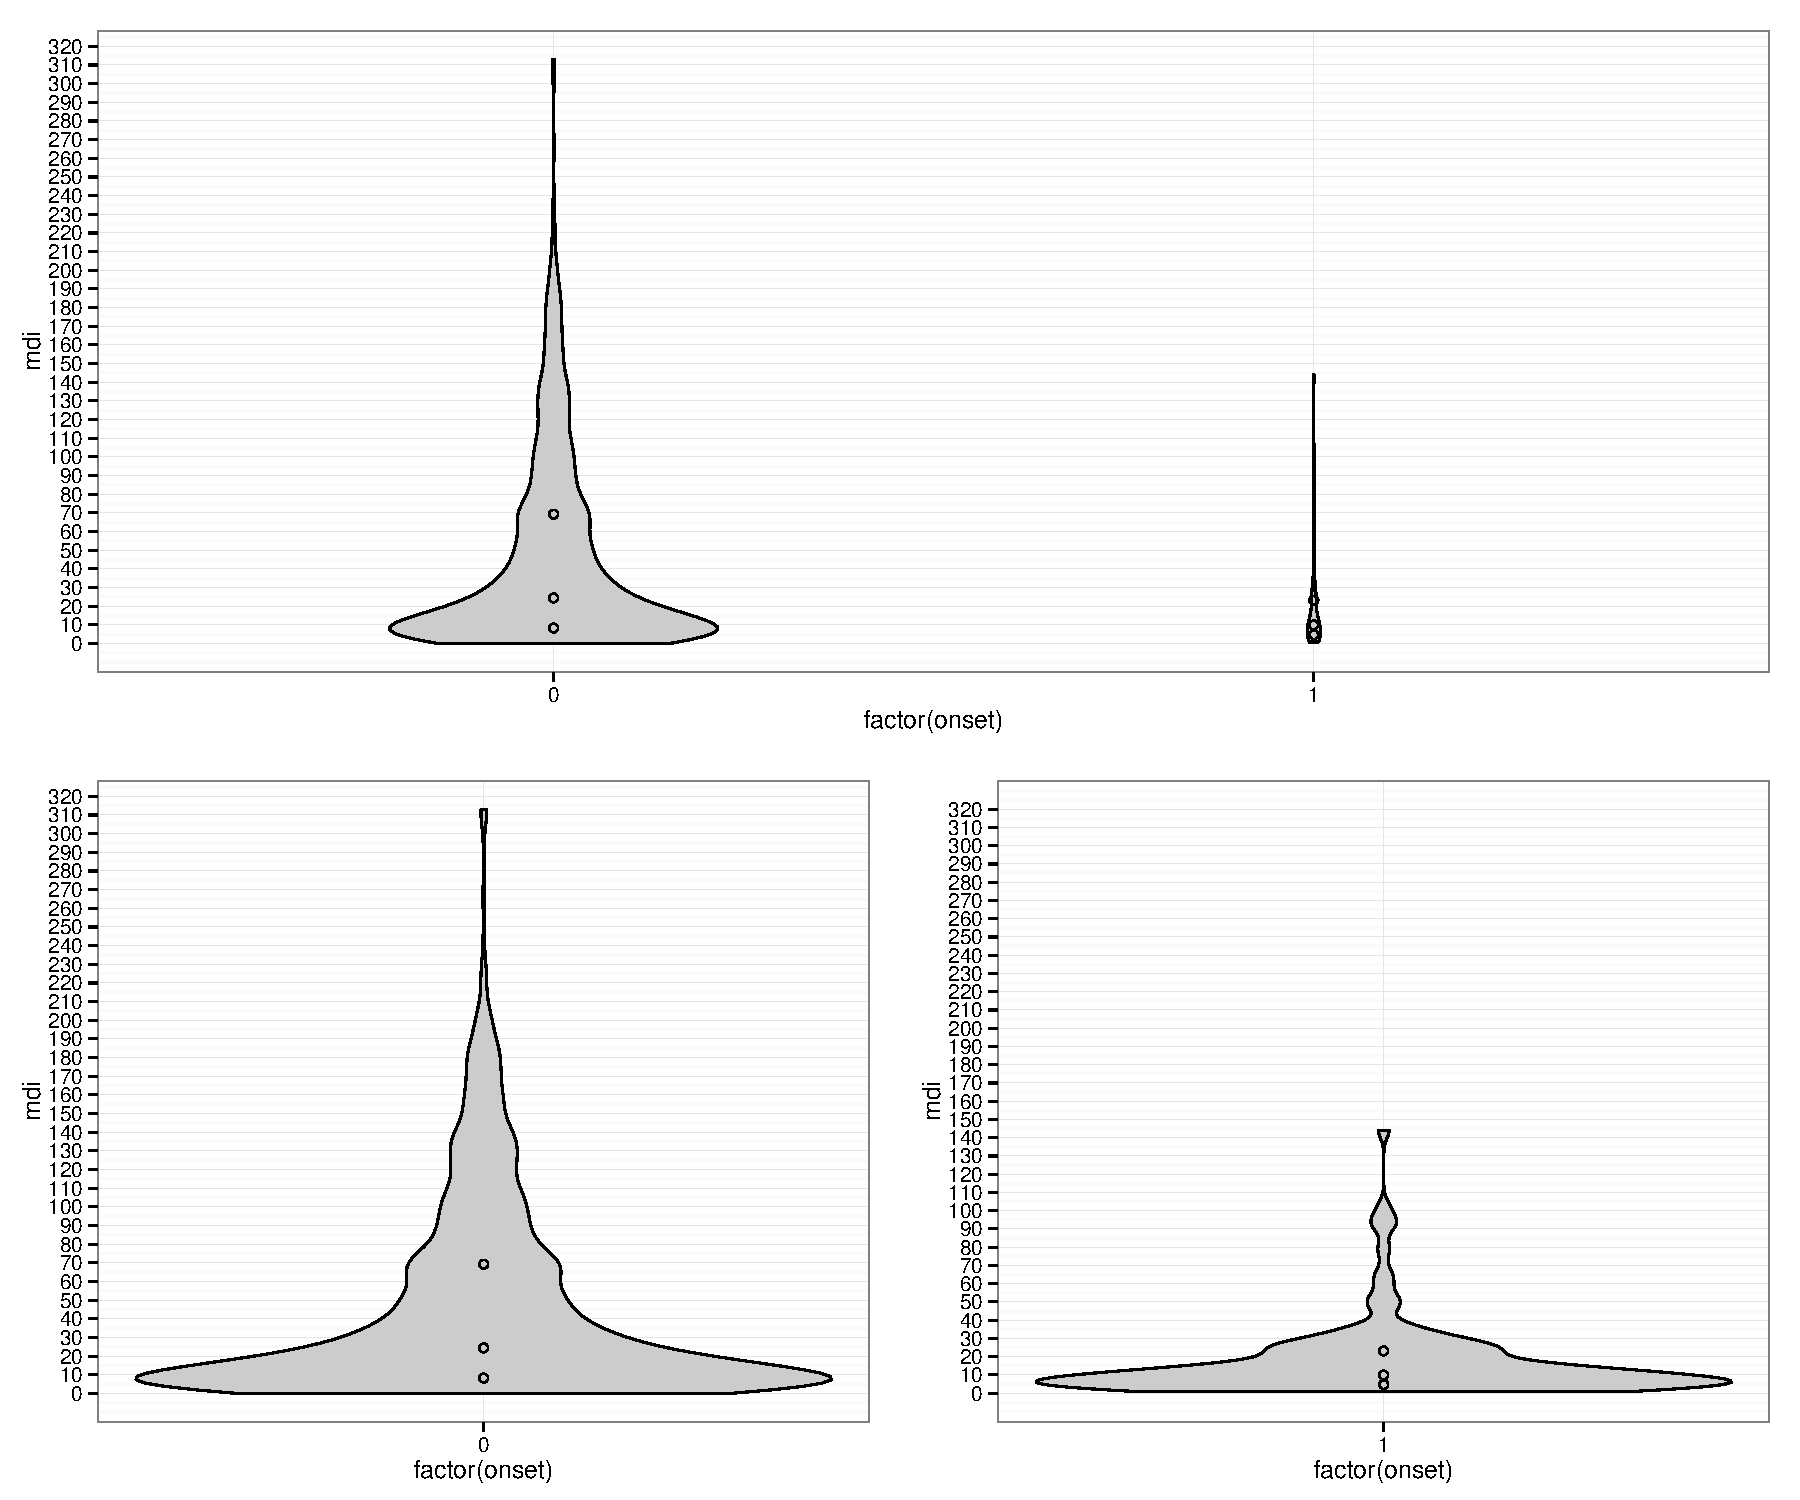
\includegraphics{figure/violinplot.pdf}
\caption{Violin plot of media density for all civil war onsets}
\end{figure}

\begin{table}[!htbp] \centering 
  \caption{Early Growth of Media Density Compared to Media Density in General} 
  \label{} 
\footnotesize 
\begin{tabular}{@{\extracolsep{5pt}}lccc} 
\\[-1.8ex]\hline \\[-1.8ex] 
\\[-1.8ex] & \multicolumn{3}{c}{onset} \\ 
\\[-1.8ex] & (1) & (2) & (3)\\ 
\hline \\[-1.8ex] 
 mdi & $-$0.03$^{***}$ &  &  \\ 
  & (0.01) &  &  \\ 
  ld.mdi &  & 0.51$^{**}$ &  \\ 
  &  & (0.26) &  \\ 
  ld.news &  &  & 1.44$^{*}$ \\ 
  &  &  & (0.75) \\ 
  ld.radio &  &  & 0.27 \\ 
  &  &  & (0.31) \\ 
  ld.tv &  &  & 2.10$^{*}$ \\ 
  &  &  & (1.22) \\ 
  lgdpl & $-$0.04 & $-$0.49 & $-$0.49 \\ 
  & (0.17) & (0.32) & (0.31) \\ 
  larea & $-$0.09 & 0.01 & 0.001 \\ 
  & (0.09) & (0.15) & (0.15) \\ 
  lmtn & 0.11$^{*}$ & 0.12 & 0.11 \\ 
  & (0.06) & (0.09) & (0.09) \\ 
  lpopl & 0.27$^{***}$ & 0.28$^{**}$ & 0.28$^{**}$ \\ 
  & (0.09) & (0.13) & (0.13) \\ 
  oil2l & 0.76$^{***}$ & 1.12$^{**}$ & 1.16$^{**}$ \\ 
  & (0.28) & (0.47) & (0.48) \\ 
  deml & 0.18$^{**}$ & 0.24$^{*}$ & 0.23$^{*}$ \\ 
  & (0.08) & (0.12) & (0.12) \\ 
  deml2 & $-$0.01$^{**}$ & $-$0.01 & $-$0.01 \\ 
  & (0.003) & (0.01) & (0.01) \\ 
  ethfracl & 0.20 & $-$0.73 & $-$0.59 \\ 
  & (0.37) & (0.54) & (0.55) \\ 
  relfracl & 1.38$^{***}$ & 1.27 & 1.38$^{*}$ \\ 
  & (0.52) & (0.79) & (0.79) \\ 
  pcyrs & $-$0.06 & $-$0.10 & $-$0.10 \\ 
  & (0.09) & (0.12) & (0.12) \\ 
  spline1 & $-$0.0001 & $-$0.001 & $-$0.002 \\ 
  & (0.002) & (0.003) & (0.003) \\ 
  spline2 & $-$0.0002 & 0.0003 & 0.0004 \\ 
  & (0.001) & (0.001) & (0.001) \\ 
  spline3 & 0.0001 & 0.0000 & $-$0.0000 \\ 
  & (0.0002) & (0.0003) & (0.0003) \\ 
  Constant & $-$8.35$^{***}$ & $-$9.59$^{***}$ & $-$9.65$^{***}$ \\ 
  & (1.18) & (1.77) & (1.80) \\ 
 N & 5,899 & 1,672 & 1,672 \\ 
Log Likelihood & $-$527.50 & $-$219.80 & $-$218.40 \\ 
AIC & 1,085.00 & 469.60 & 470.70 \\ 
\hline \\[-1.8ex] 
\multicolumn{4}{l}{$^{*}$p $<$ .1; $^{**}$p $<$ .05; $^{***}$p $<$ .01} \\ 
\end{tabular} 
\end{table}

\begin{figure}[htbp]
\centering
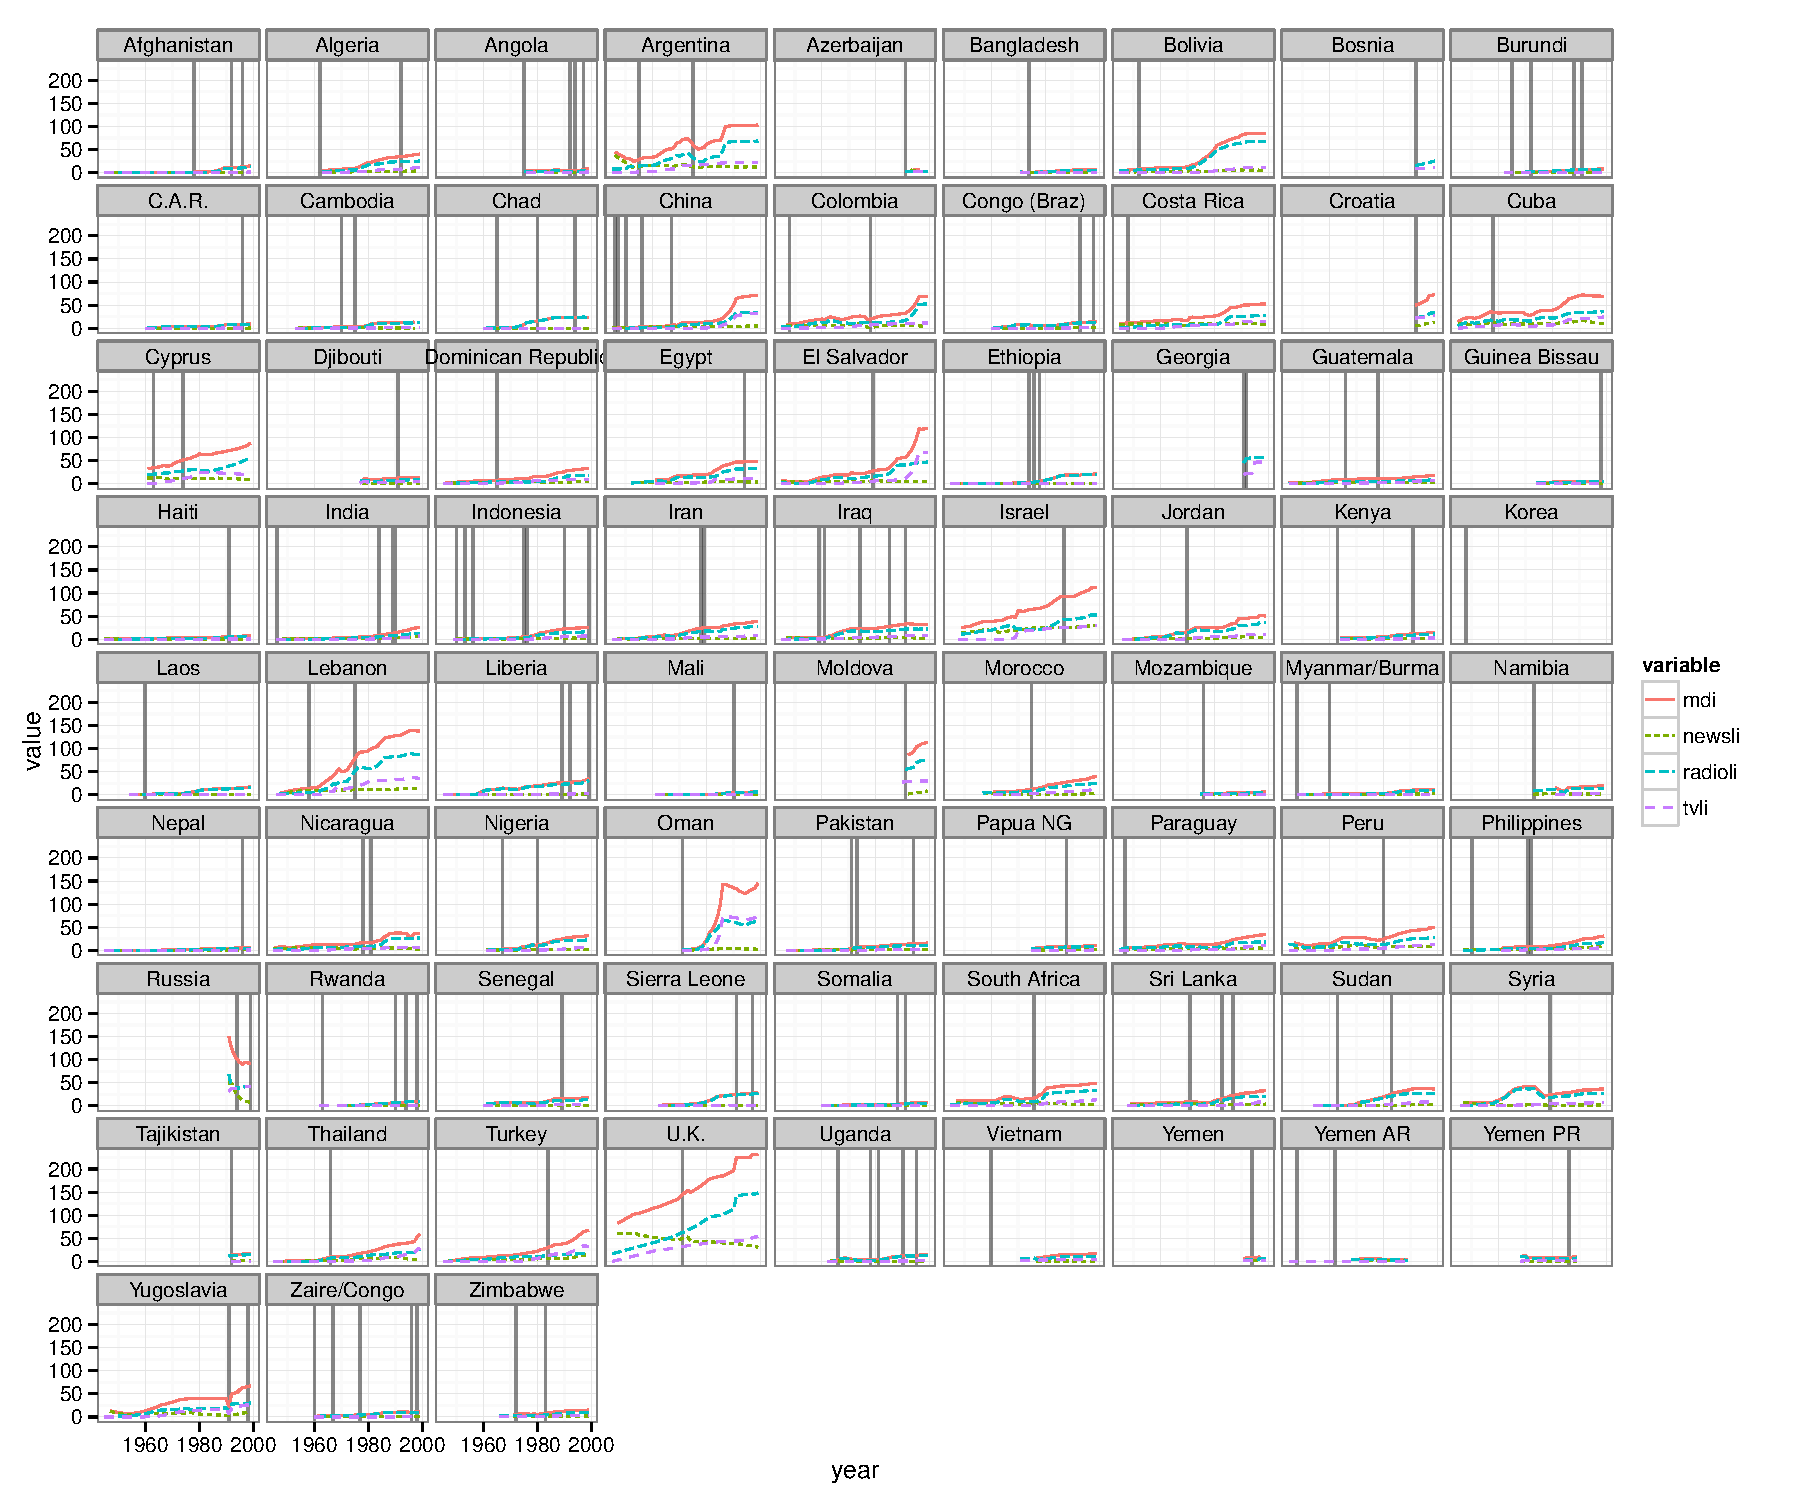
\includegraphics{figure/full_panel_plot.pdf}
\caption{Disaggregated media density and all civil war onsets over time,
by country}
\end{figure}

\section{Appendix}\label{appendix}

The Levin-Lin-Chu statistic is a standard test for the presence of a
unit root, otherwise known as non-stationarity or integration of order
I(1), in a time series variable observed across multiple cross-sectional
units. The Im-Pesaran-Shin test is a ``second generation'' test which is
robust to cross-sectional dependence, common in cross-national panel
data. For each test, the null hypothesis is the presence of a unit root.
Because the tests require balanced panels, they were applied only to the
24 countries with the maximum time-series of 55 years, a subset which
still contains significant variation in geography, income, regime type,
and other factors. Specifically, the countries in this subset are:
Canada, Cuba, Haiti, Dominican Republic, Mexico, Honduras, El Salvador,
Nicaragua, Costa Rica, Uruguay, Ireland, Netherlands, Belgium,
Luxembourg, France, Switzerland, Hungary, Romania, Finland, Sweden,
Norway, Denmark, Afghanistan, China.

\begin{verbatim}
Levin-Lin-Chu Unit-Root Test (ex. var. : Individual Intercepts
and Trend )
\end{verbatim}

data: unit\$mdi z.x1 = -0.3222, p-value = 0.7473 alternative hypothesis:
stationarity

\begin{verbatim}
Pesaran's CIPS test for unit roots
\end{verbatim}

data: unit\$mdi CIPS test = -2.064, lag order = 2, p-value = 0.1
alternative hypothesis: Stationarity

\pagebreak   

\section*{References}\label{references}
\addcontentsline{toc}{section}{References}

\setlength{\parindent}{-0.2in} \setlength{\leftskip}{0.2in}
\setlength{\parskip}{8pt} \vspace*{-0.2in} \noindent

Im, Kyung So, M Hashem Pesaran, and Yongcheol Shin. 2003. ``Testing for
Unit Roots in Heterogeneous Panels.'' \emph{Journal of Econometrics}
115(1): 53--74.
\url{http://linkinghub.elsevier.com/retrieve/pii/S0304407603000927}.

Levin, Andrew, Chien-Fu Lin, and Chia-Shang James Chu. 2002. ``Unit Root
Tests in Panel Data: Asymptotic and Finite-Sample Properties.''
\emph{Journal of Econometrics} 108(1): 1--24.
\url{http://linkinghub.elsevier.com/retrieve/pii/S0304407601000987}.

Warren, T Camber. 2014. ``Not by the Sword Alone: Soft Power, Mass
Media, and the Production of State Sovereignty.'' \emph{International
Organization} 68(01): 111--41.
\url{http://www.journals.cambridge.org/abstract_S0020818313000350}.


\end{document}